 \documentclass[12pt,a4paper]{report}
 \usepackage[dvipdfmx]{graphicx}
 \usepackage{listings}
 \usepackage[pdftex]{hyperref}
 \usepackage{url}
 \usepackage{graphicx,color}
 \usepackage[font=scriptsize]{caption}
 \usepackage{subcaption}
 \usepackage{fullpage}
 \usepackage{footnote}
 \usepackage{pdfpages}
 \usepackage{amsmath}
 \usepackage{longtable}
 \usepackage{tcolorbox}

 \newcommand\tab[1][0.5cm]{\hspace*{#1}}
 \newcommand{\command}[1]{\textcolor{blue}{#1}}
 \newcommand{\titulo}{{\bf Lab Book}\\{\it project title}\\Author}
 \newcommand{\autor}{Advisor\\Institute}


\title{\titulo}
\author{\autor}
\date{2023}

 \begin{document}
 \maketitle
 %\listoffigures - List the figures
 %\listoftables - List the tables
 \tableofcontents
 \newpage

%%%%%%%%%%%%%%%%%%%%%%%%%%%%%%%%%%%%%%%%%%%%%%%%%%%%%
%%%%%%%%%%%%%%%%%%%%%%%%%%%%%%%%%%%%%%%%%%%%%%%%%%%%%

 \chapter{March 2023}
 
 \section{13 - Work organization}
 In bioinformatics and computational biology it is extremely important to organize your files, scripts, reports, among others. In table~\ref{aspects}, I mention the most important aspects that should be addressed in your organization and helpful tools. \\
 
 In summary, you need an adequate tool for each aspect, say latex or word for project documentation, and a backup and/or version control tool, say GIT or a cloud option for project documentation.

\begin{table}[!htb]
  \caption{Aspects of organization and respective tools.}
  \label{aspects}
  \centering
  \begin{tabular}{cc}
  \hline 
	Aspect&Tools and backup \\
  \hline
       Project documentation&Latex \& GIT; word \& cloud; google docs  \\
       Scripts& GIT; cloud \\
       Papers, reports and presentations& Latex \& GIT; word \& cloud; google docs \\
       Bibliography& Latex; Citavi, etc. \\
  \hline
  \end{tabular}
 \end{table}
 
 \subsection{Learning Latex}
 \hspace{0.2cm}
 \begin{tcolorbox}[width=6.3in]
 \scriptsize 
 - Working folder: \textit{path}
 
 - Source: \url{https://github.com/waltercostamb/Lab-Book}
 \end{tcolorbox}
 \hspace{0.2cm}
 \normalsize  
 
  \LaTeX{} is a high-quality typesetting system, available as free software, which allows to produce scientific or technical documents \cite{latex-main}. I am using \LaTeX{} to create a Bioinformatics Lab Book. To compile my Lab Book, I can use command lines (\command{pdflatex} and \command{bibtex}). Afterwards I can visualise the produced {\it .pdf} file with evince or another reader. Alternatevily, I can use a Latex editor, such as TexWorks (\url{https://www.tug.org/texworks/}), which allows me to write the code and control the {\it pdf} file in the same environment (Figure~\ref{texworks}).  \\
  
 % \newpage
  
  To compile the {\it .tex} file in the command line: \\
  
  \command{\$pdflatex lab-book}
  
  \command{\$bibtex lab-book}
  
  \command{\$pdflatex lab-book}
    
  \command{\$pdflatex lab-book} \\
  
   To visualise the {\it .pdf}: \\
  
  \command{\$evince lab-book.pdf \&}
  
    \begin{figure}
  \centering 
  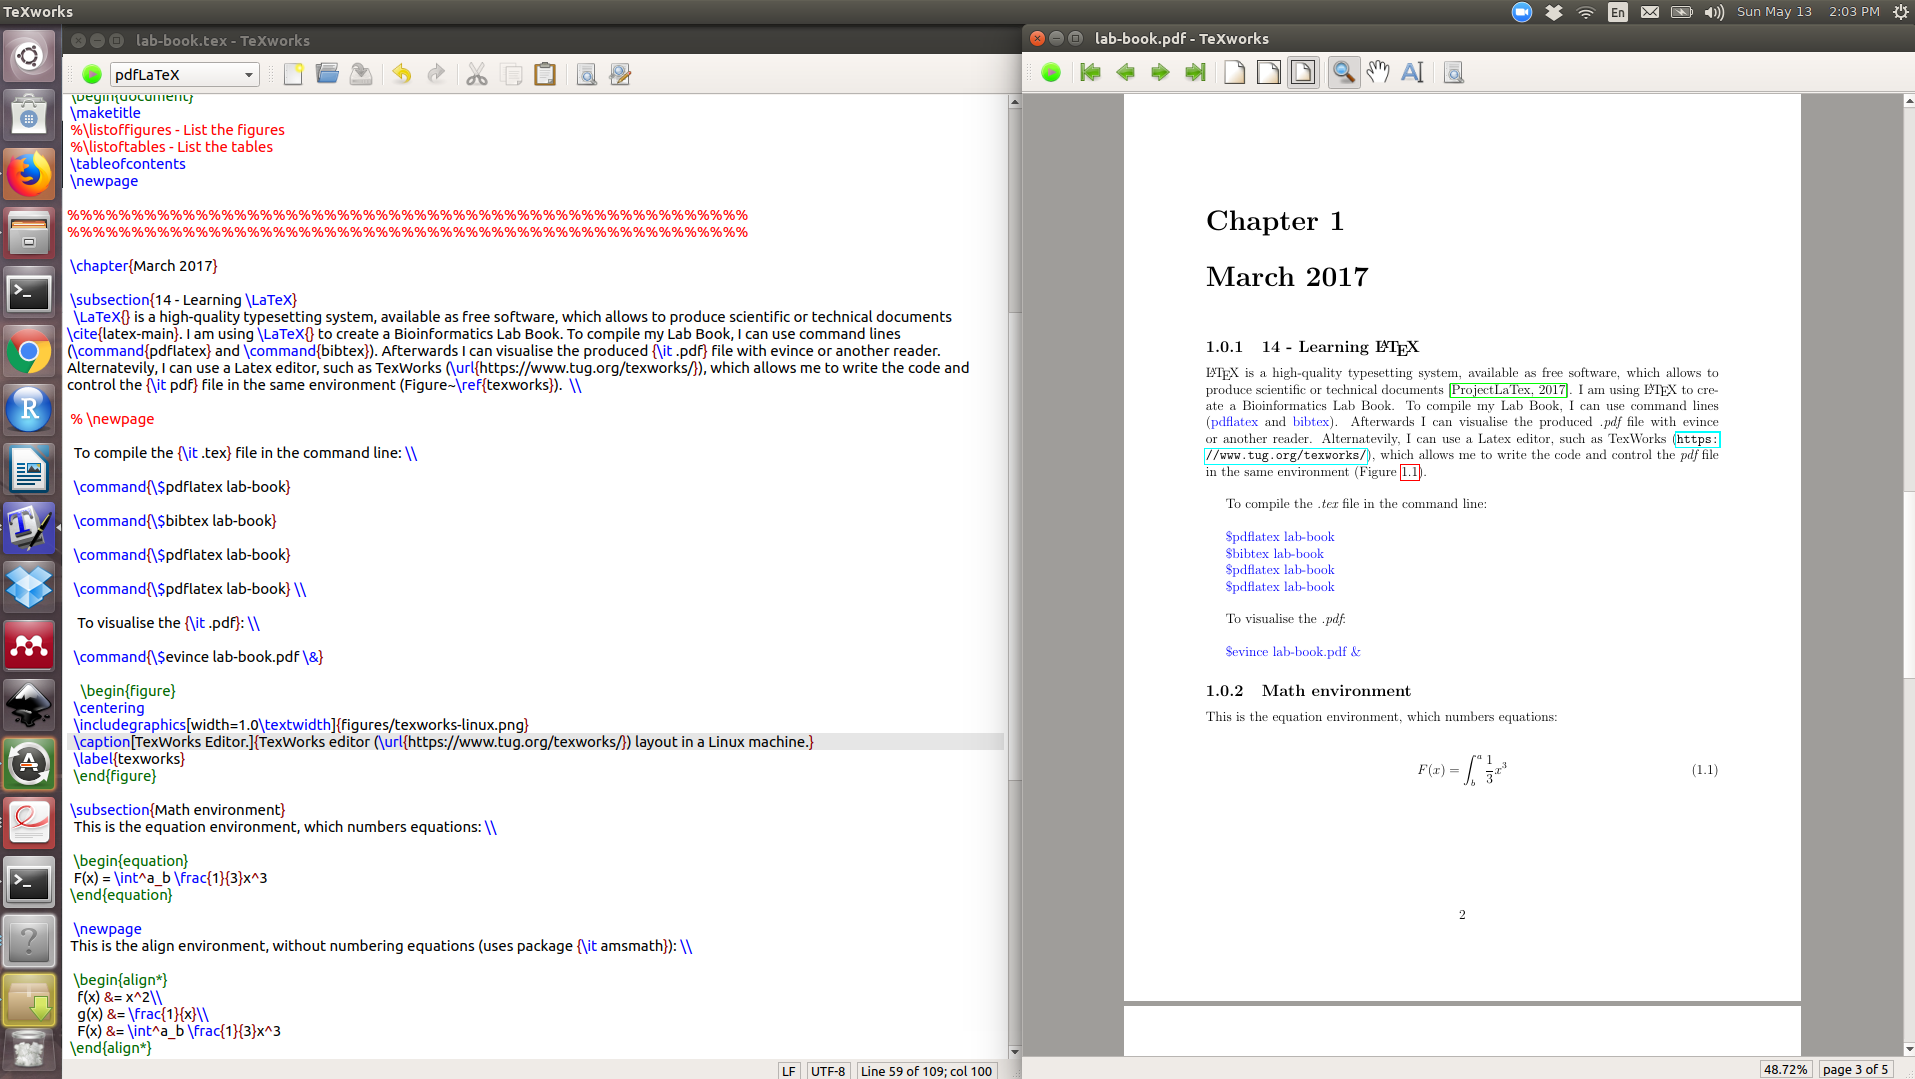
\includegraphics[width=1.0\textwidth]{figures/texworks-linux.png} 
  \caption[TexWorks Editor.]{TexWorks editor (\url{https://www.tug.org/texworks/}) layout in a Linux machine.}
  \label{texworks} 
  \end{figure}
  
 \subsubsection{Math environment}
  This is the equation environment, which numbers equations: \\
  
  \begin{equation}
  F(x) = \int^a_b \frac{1}{3}x^3
 \end{equation}
 
%\newpage
 This is the align environment, without numbering equations (uses package {\it amsmath}): \\
 
  \begin{align*}
   f(x) &= x^2\\
   g(x) &= \frac{1}{x}\\
   F(x) &= \int^a_b \frac{1}{3}x^3
 \end{align*}
 
  \section{14 - Project proposal}
 Some text here. Incluing and referencing a table (table~\ref{table1}).
 
 \begin{itemize}
\item First numbered list item
\item Second numbered list item
\end{itemize}

\begin{table}[!htb]
  \caption{Descriptio of table 1.}
  \label{table1}
  \centering
  \begin{tabular}{ccc}
  \hline 
       species&changes&score \\
  \hline
       Macaque&4&0.0 \\
       Human&2&14.9 \\
       Orangutan&0&0.0 \\
       Pan&0&0.0 \\
       Gorilla&0&0.0 \\
  \hline
  \end{tabular}
 \end{table}
 
 
 \bibliographystyle{apalike}
 \bibliography{ref}


 \end{document}
